\section{Results and Discussion}

\subsection*{Public Dataset: COLO}

The COLO dataset contains 1254 images and 11818 cow instances captured from an indoor farm environment. The dataset is organized in YOLO and COCO formats and published on the online platforms GitHub \href{https://github.com/Niche-Squad/COLO/}{(https://github.com/Niche-Squad/COLO/)} and Huggingface \href{https://huggingface.co/datasets/Niche-Squad/COLO}{(https://huggingface.co/datasets/Niche-Squad/COLO)}. The dataset consists of eight configurations (\textbf{Table~\ref{tab:colo_config}}):
\textit{0\_all}, \textit{1\_top}, \textit{2\_side}, \textit{3\_external}, \textit{a1\_t2s}, \textit{a2\_s2t}, \textit{b\_light}, and \textit{c\_external}. The \textit{0\_all} configuration serves as the baseline for this study, featuring non-overlapping training and testing images collected from both the Top-View Camera and Side-View Camera. The \textit{1\_top}, \textit{2\_side}, and \textit{3\_external} configurations contain images from their respective cameras. The \textit{a1\_t2s}, \textit{a2\_s2t}, and \textit{b\_light} configurations include training/testing splits for the Top2Side, Side2Top, and Day2Night scenarios, respectively. The \textit{c\_external} configuration features training images from the Top-View and Side-View Cameras, with testing images from the External Camera. The dataset hosted on GitHub is available as a compressed zip file for public access. In contrast, the dataset on Huggingface requires the Python package "datasets" \cite{datasets} to download. The Huggingface version offers additional functionality to resize the images and annotations to specific resolutions, providing greater flexibility for various applications.

\begin{table}[h]
    \caption{Description of the COLO dataset configurations.}
    \centering
    \begin{tabular}{lll}
        \toprule
        \textbf{Configuration} & \textbf{Training Samples} & \textbf{Testing Samples} \\
        \midrule
        \textit{0\_all} & Top-View + Side-View & Top-View + Side-View \\ [0.5ex]
        \textit{1\_top} & Top-View & Top-View \\[0.5ex]
        \textit{2\_side} & Side-View & Side-View \\[0.5ex]
        \textit{3\_external} & External & External \\[0.5ex]
        \midrule
        \textit{a1\_t2s} & Top-View & Side-View \\[0.5ex]
        \textit{a2\_s2t} & Side-View & Top-View \\[0.5ex]
        \textit{b\_light} & Day & Night \\[0.5ex]
        \textit{c\_external} & Top-View + Side-View & External \\[0.5ex]
        \bottomrule
    \end{tabular}
    \label{tab:colo_config}
\end{table}

\subsection*{Evaluation Metrics}

To assess the performance of the YOLO models, we used four key metrics: $\text{mAP@{0.5:0.95}}$, $\text{mAP@{0.5}}$, precision, and recall. These metrics provide a comprehensive understanding of how well the models detect and localize cows in the images from the COLO dataset. A pair-wise comparison of these metrics is presented in \textbf{Figure~\ref{fig:metrics}} to illustrate their interrelationships.

The $\text{mAP@{0.5:0.95}}$ metric is the most stringent, requiring the model to achieve both high positioning accuracy (i.e., high IoU) and high precision across IoU thresholds from 0.5 to 0.95. Because it is less likely to be influenced by high-confidence predictions alone, it serves as a reliable indicator of overall model performance. Achieving an accuracy greater than 0.90 on this metric is generally unrealistic; typically, a value of 0.7 is considered good and is sufficient to yield precision and recall of around 0.9.

In contrast, $\text{mAP@{0.5}}$ is more lenient, requiring high confidence but only moderate IoU. It measures the average precision at an IoU threshold of 0.5. For applications where counting cows is more important than precise positioning, an $\text{mAP@{0.5}}$ value of 0.9 is sufficient. For example, our results showed that the YOLOv8n model, trained on 32 samples, achieved an $\text{mAP@{0.5}}$ of 0.9, making it suitable for such applications.

Precision and recall metrics focus on the accuracy and completeness of the detections. Precision is the ratio of true positive detections to the total number of positive detections (true positives + false positives), measuring how accurate the positive predictions are. Recall is the ratio of true positive detections to the total number of actual positives (true positives + false negatives), measuring the model’s ability to detect all relevant objects. Generally, higher precision is associated with higher recall. However, in some configurations, such as Side2Top and External with smaller sample sizes, models exhibited high recall but low precision. This indicates a tendency to misclassify non-cow objects as cows more frequently than missing actual cows, suggesting a tendency to overestimate rather than underestimate the number of cows in the images.

Our observations emphasize that for applications where counting cows is more critical than precise positioning, achieving a high $\text{mAP@{0.5}}$ is adequate, while the stringent $\text{mAP@{0.5:0.95}}$ metric serves as a comprehensive indicator of overall model performance. These metrics provide insights into both the localization and classification capabilities of the models, helping to identify strengths and weaknesses under different environmental conditions and camera angles.

\begin{figure}[h]
    \centering
    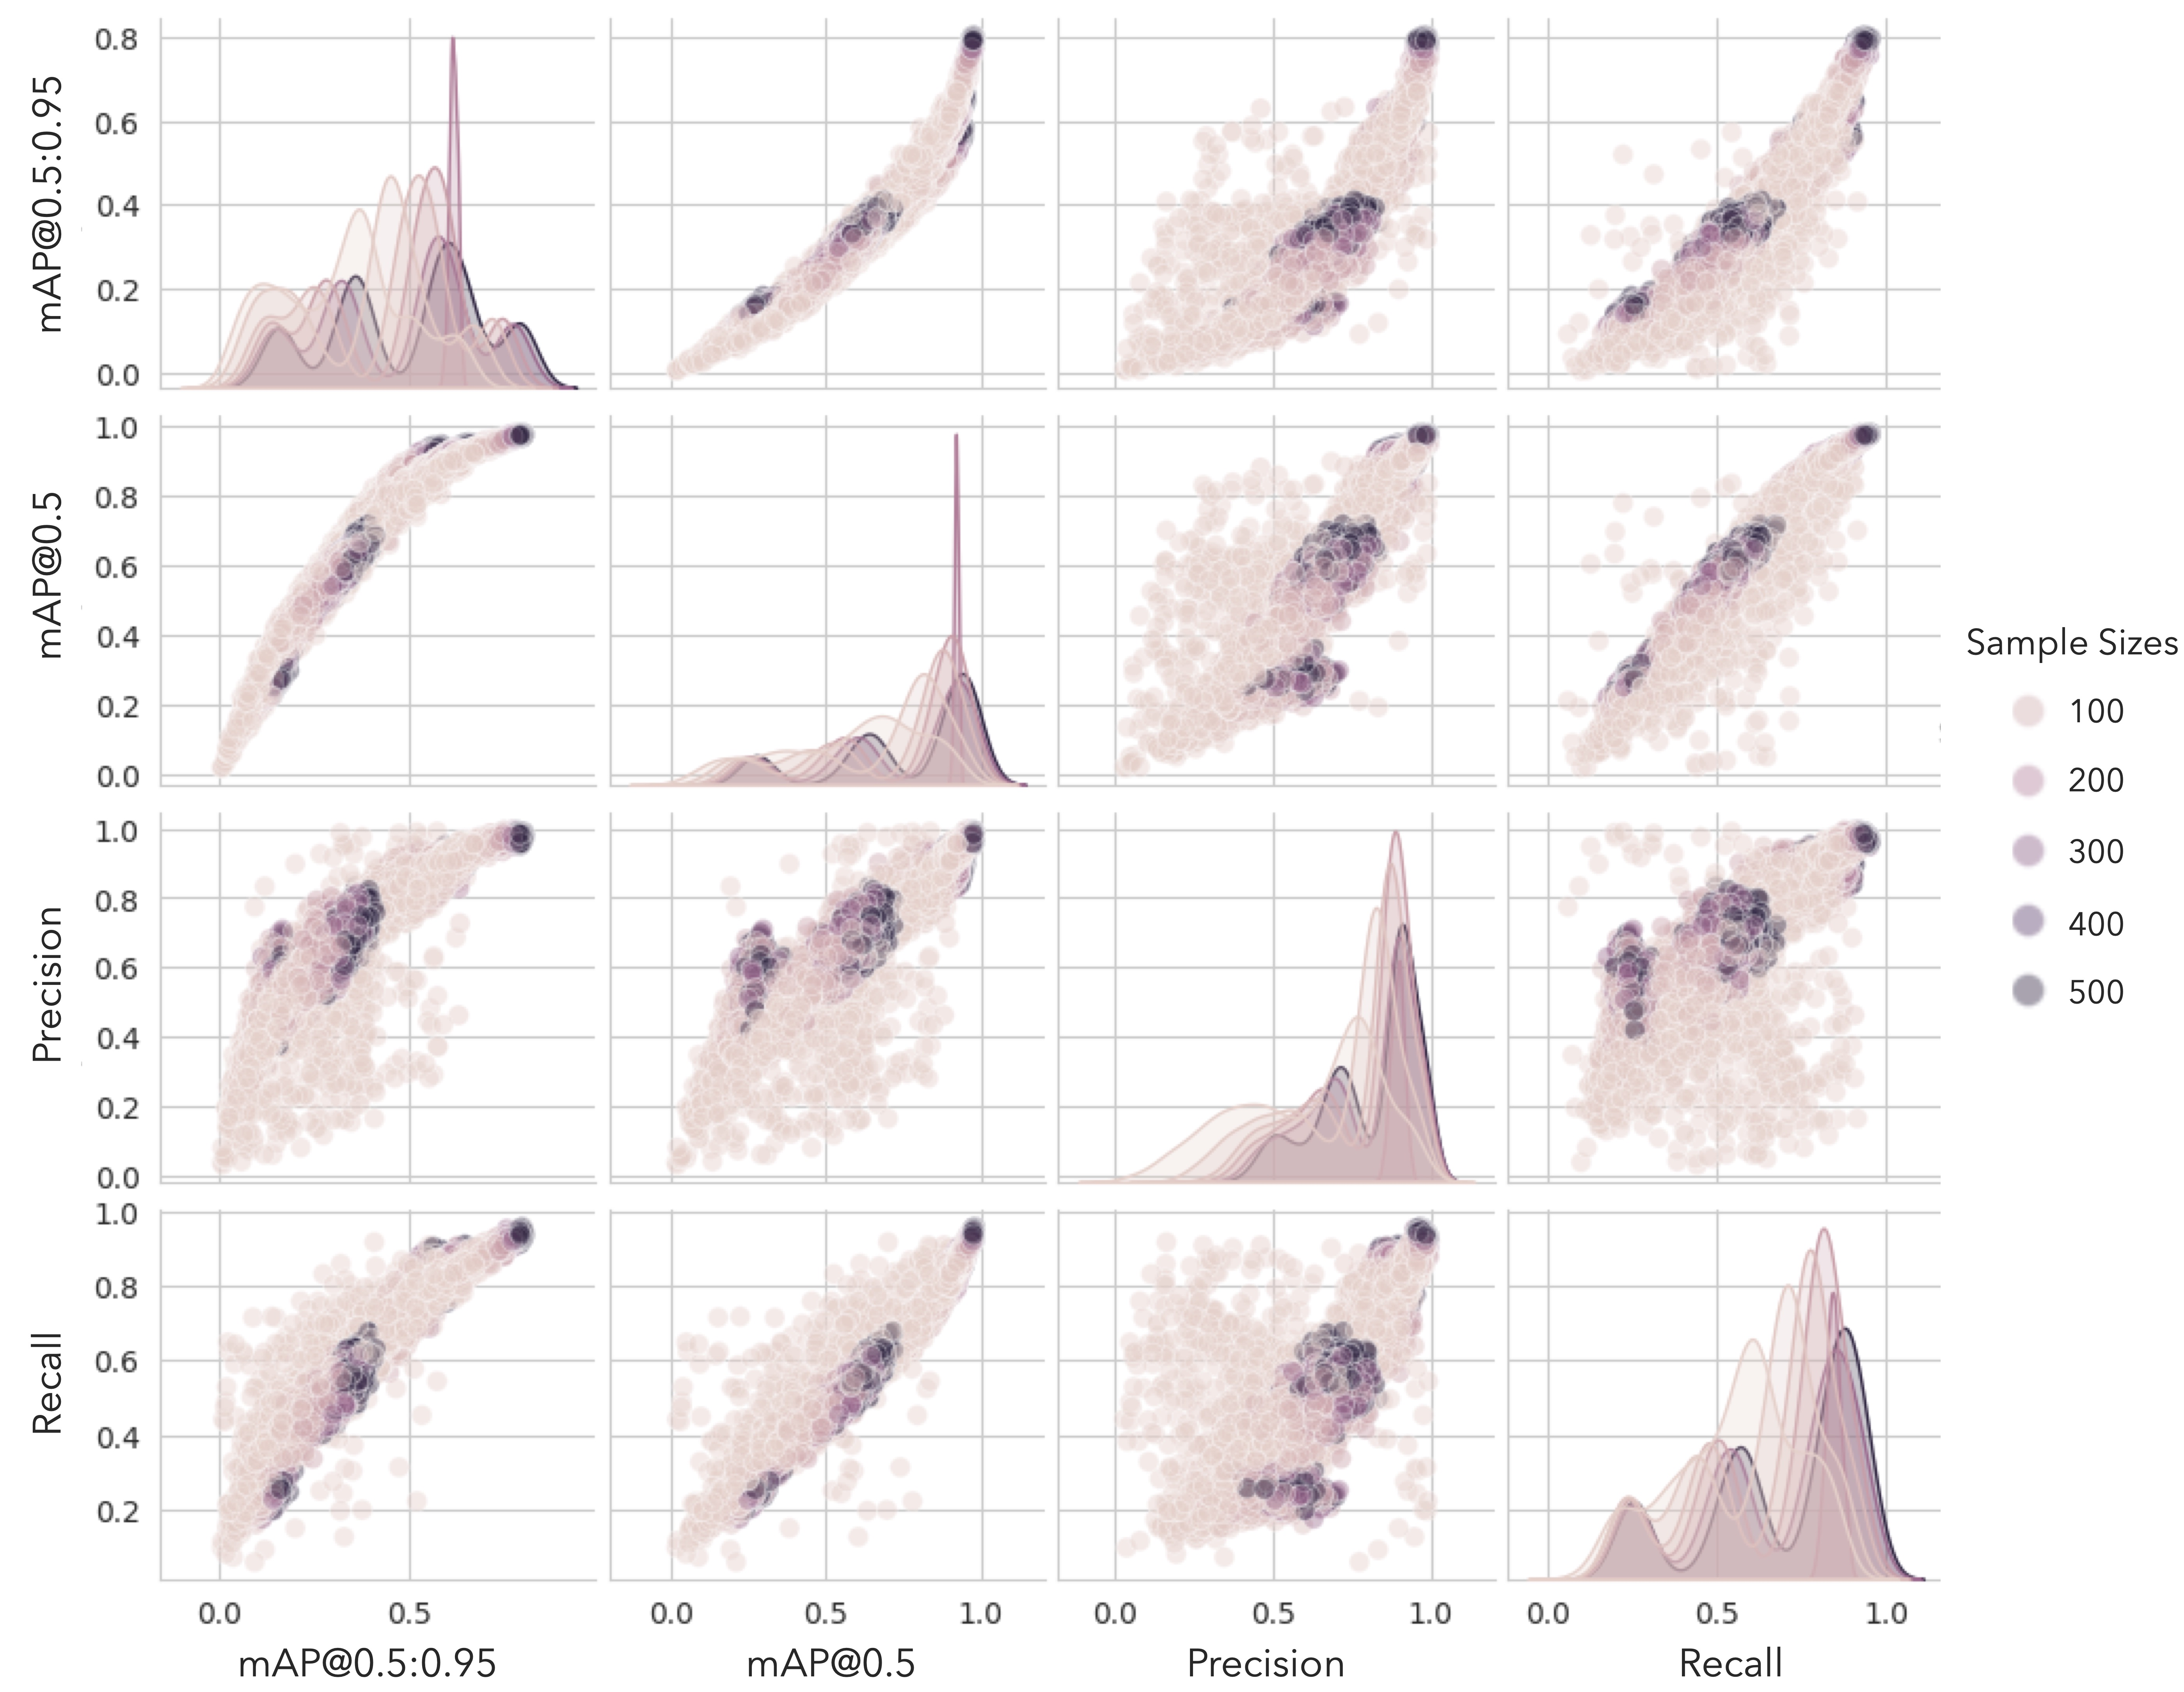
\includegraphics[width=1\textwidth]{figure_s1.jpg}
    \caption{Pairwise scatter plots of the evaluation metrics: $\text{mAP@{0.5:0.95}}$, $\text{mAP@{0.5}}$, precision, and recall. Each point represents a different model configuration, with the color indicating the training sample size.}
    \label{fig:metrics}
\end{figure}

\subsection*{Study 1: The Changes in Camera View Angles Dramatically Affect Model Performance}

The baseline training configuration showed good generalization capability, with over 90\% of the predictions correctly positioning cows at the 50\% IoU criterion ($\text{mAP@{0.5}}$). The generalization performance can be dissected into changes in view angles (i.e., Top2Side and Side2Top) and lighting conditions (i.e., Day2Night). Changes in lighting conditions did not dramatically affect model performance across all four metrics. However, changing camera views resulted in a performance drop of approximately 30\% and 60\% in $\text{mAP@{0.5}}$ for the Side2Top and Top2Side configurations, respectively. Across all metrics and training sample sizes, the Top2Side configuration consistently showed the worst performance.

\begin{figure}[h]
    \centering
    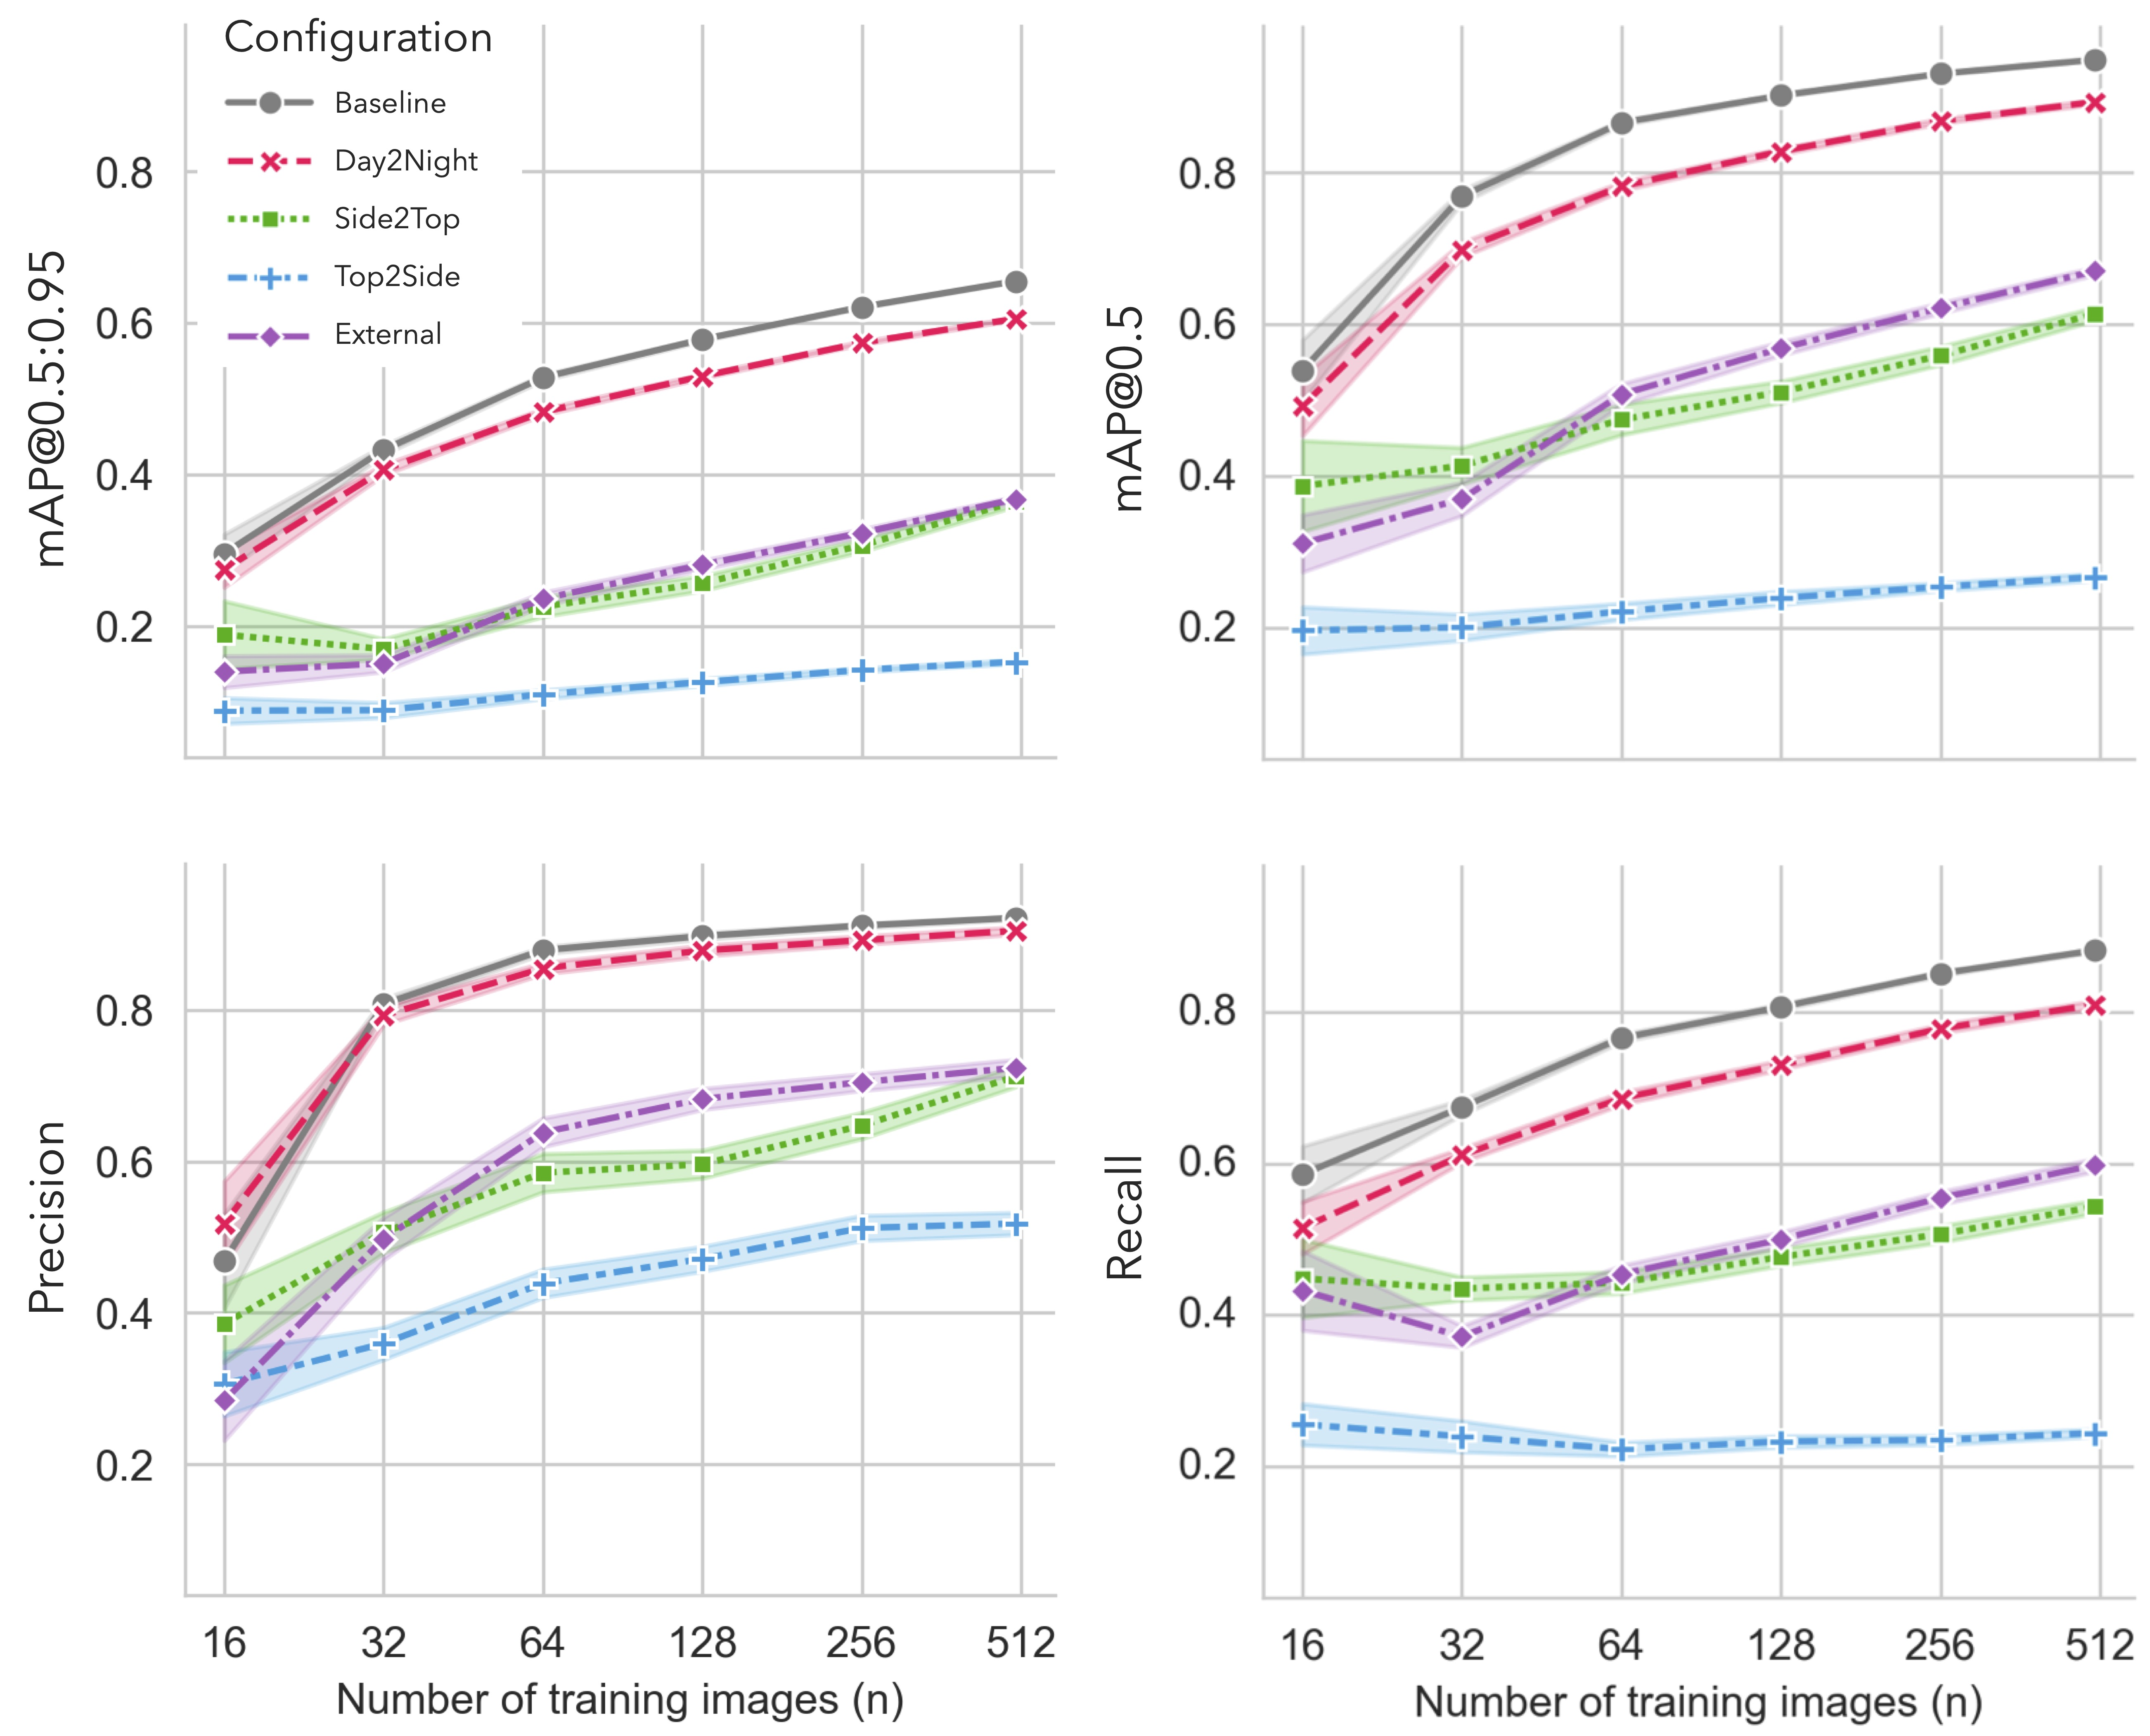
\includegraphics[width=0.8\textwidth]{figure_3.jpg}
    \caption{The generalization performance of YOLOv9e across various data configurations and training sample sizes. Sample sizes are depicted on the horizontal axis using a logarithmic scale with a base of 2, and the data configurations are represented by different colors and marker shapes. The upper left and right plots display the metrics $\text{mAP@{0.5:0.95}}$ and $\text{mAP@{0.5}}$, respectively, for different training samples across diverse data configurations. The lower left and right plots depict precision and recall values, also for varying training samples and configurations.}
    \label{fig:schemes}
\end{figure}

From the perspective of precision and recall, changing the camera view from Top2Side resulted in the model missing more than 7 out of every 10 cows, with only 50\% of the detections being correct. For the 'External' configuration, our model identified 6 out of every 10 cows, which is not ideal but also not the worst performance observed. Notably, performance in the Day2Night configuration was close to the baseline in terms of precision, which only considers predictions with high confidence compared to $\text{mAP@{0.5}}$. Hence, by excluding low-confidence predictions, changes in lighting conditions did not affect model performance. Regardless of the configuration and evaluation metrics, model performance always increased as the training sample sizes increased.

This study provides a comparative analysis of the behavior of the model in various data configurations. It is clear that the `Day2Night' configuration shows much better performance relative to the heterogeneous viewpoint-oriented configurations `Top2Side' and `Side2Top'.

Despite the various challenges in adapting models from day to night conditions, the `Day2Night' configuration consistently maintains high precision, closely mirroring the `Baseline' configuration across all training sample sizes. This suggests that changes in lighting have less impact on the model's ability to detect objects compared to changes in viewpoint. This robustness to lighting could be attributed to the inclusion of diverse lighting conditions in the training phase. Specifically, model performance benefited from pixel-wise augmentation techniques such as adjustments to hue, saturation, and value (HSV). These augmentations introduced a variety of color variations to the images, enhancing the model's ability to generalize across different visual conditions. Moreover, these YOLO models benefit from pre-training on the COCO dataset, which is characterized by a wide array of images with varied lighting, aiding their adaptability to shifts in light.

On the other hand, the models perform suboptimally in scenarios involving changes in viewpoint. Each new viewpoint introduces fundamentally different object features that are not replicated through standard data augmentation methods such as lighting or affine transformations. For example, when the camera is placed at a lower angle, cows are more frequently occluded by stalls and fences. These additional objects introduce variations that cannot be mitigated by augmentations in HSV space or image translation. Consequently, `Top2Side' performs the worst, as it is particularly challenging to identify cows from the side. Even for the `External' configuration, the model struggles to generalize well despite being trained on the `Baseline' configuration because the camera angle is changed again in the `External' setup. In summary, camera view angle is crucial for model generalization, with side views being the most challenging.

\subsection*{Study 2: A Higher Model Complexity Does Not Always Lead to Better Performance}

\begin{figure}[h]
\centering
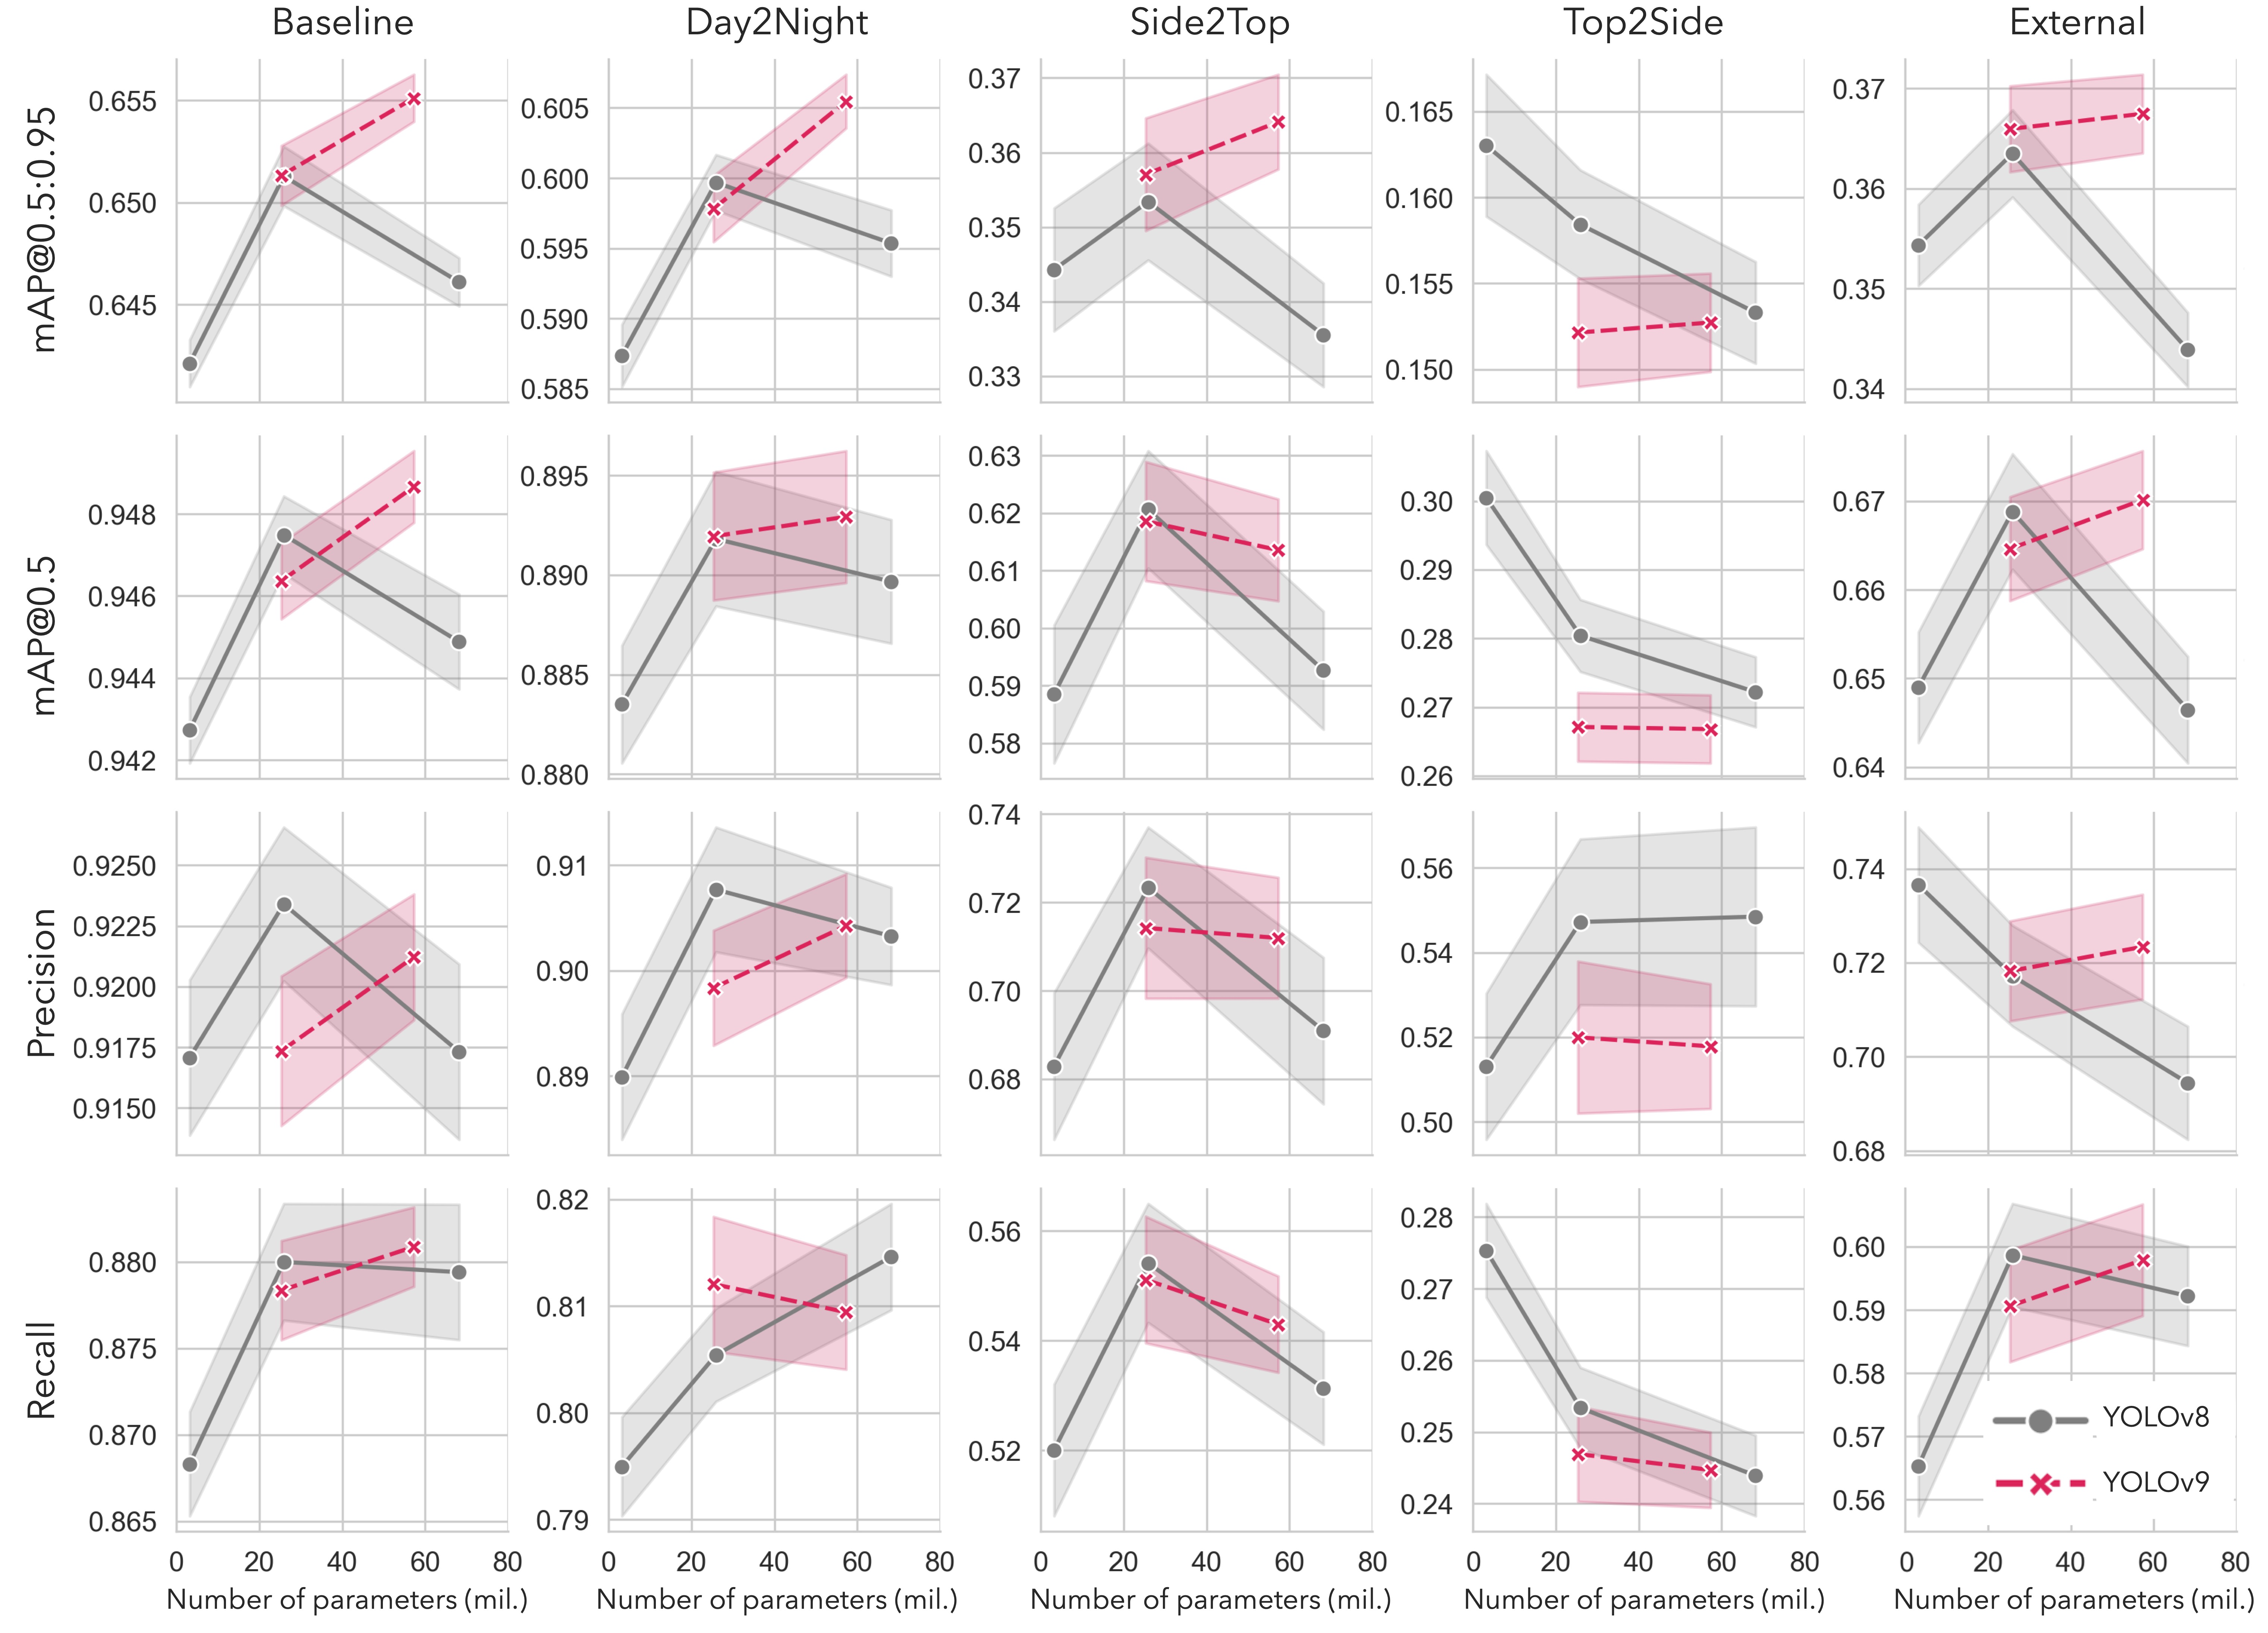
\includegraphics[width=1\textwidth]{figure_4.jpg}
\caption{The performance of YOLOv8 and YOLOv9 models across various model parameters and data configurations, evaluated using four metrics: $\text{mAP@{0.5:0.95}}$, $\text{mAP@{0.5}}$, precision, and recall. Each column indicates a different data configuration, starting from top left to bottom right: `Baseline', `Day2Night', `Side2Top', `Top2Side', and `External'. The horizontal axis of all plots indicates the number of model parameters.}
\label{fig:models}
\end{figure}

The study found that the training configuration significantly affects the relationship between model complexity and performance. Based on Study 1, predicting images from a side view using a model trained on Top-View camera images is one of the most challenging tasks. In this configuration, increasing model complexity generally resulted in poorer generalization, with simpler models often performing better. However, in other configurations that demonstrated better generalization in Study 1, the peak performance was not always achieved by the most complex model. For example, in the baseline configuration, the YOLOv9e model performed best in terms of $\text{mAP@{0.5:0.95}}$, $\text{mAP@{0.5}}$, and recall, while the YOLOv8m model excelled in precision. Neither of these models had the highest parameter counts compared to YOLOv8x. It is also worth noting that different model architectures showed different performance trends with varying complexities. The YOLOv8-family models tended to perform best with mid-sized models (i.e., YOLOv8m), whereas larger models in the YOLOv9 family usually performed better. Hence, the study concluded that model performance is determined by both the training configuration and the model architecture.

The study results, as shown in \textbf{Figure \ref{fig:models}}, indicate that although both YOLOv8 \cite{ultralyticsYOLOv8} and YOLOv9 \cite{wang2024yolov9} models exhibit an increase in $\text{mAP@{0.5}}$ with more parameters when trained on the COCO dataset \cite{lin2014microsoft}, this does not support a definitive conclusion that more parameters consistently improve model performance. This may be because the prior work's findings were based on the COCO dataset, which includes 80 classes and mainly features standalone images. In contrast, this study uses an indoor farm dataset focused exclusively on a single class: cows. Consequently, the model may not need as many parameters to effectively detect cows. This suggests that researchers should not rely solely on public dataset performance, as model generalization is specific to the task and dataset.

Additionally, this study found that a small model such as YOLOv8n, with only 3.2M parameters, can yield 90\% accuracy with a relatively small size of training samples. This indicates that when one encounters a simple and homogenous task like positioning cows, deploying a small model is optimal in balancing computing time and prediction accuracy. This further underscores the importance of considering the specific characteristics of the task and dataset when choosing a model, rather than defaulting to more complex models under the assumption they will perform better.

Overall, our findings emphasize that higher model complexity does not necessarily lead to better performance. The optimal model configuration depends heavily on the specific task and dataset, highlighting the need for careful model selection tailored to the particular application at hand.

\subsection*{Study 3: The Advantages of Custom Initial Weights are Limited When the Model is Simple}

The results presented in Figure \ref{fig:finetune} indicate that the benefit of using fine-tuned initial weights is minimal for simpler models. Specifically, when employing YOLOv8n, the performance difference between the default and fine-tuned weights was insignificant when fine-tuning data from the Top-View Camera and Side-View Camera. However, as model complexity increased, a greater number of fine-tuning samples were required for the two different initial weights to achieve similar performance. For instance, in the case of YOLOv9e, the performance gap was eliminated when the number of fine-tuning samples reached 128 and 64 for the Top-View Camera and Side-View Camera data sources, respectively. A similar trend was observed with the External camera, where a significant performance gap of more than 25\% in $\text{mAP@{0.5:0.95}}$ was observed for YOLOv9e when the sample size was 16. It is also noted that, although the performance gap was closed to zero for the Top-View Camera and Side-View Camera data sources, the gap was never closed for the External camera.

\begin{figure}[h]
    \centering
    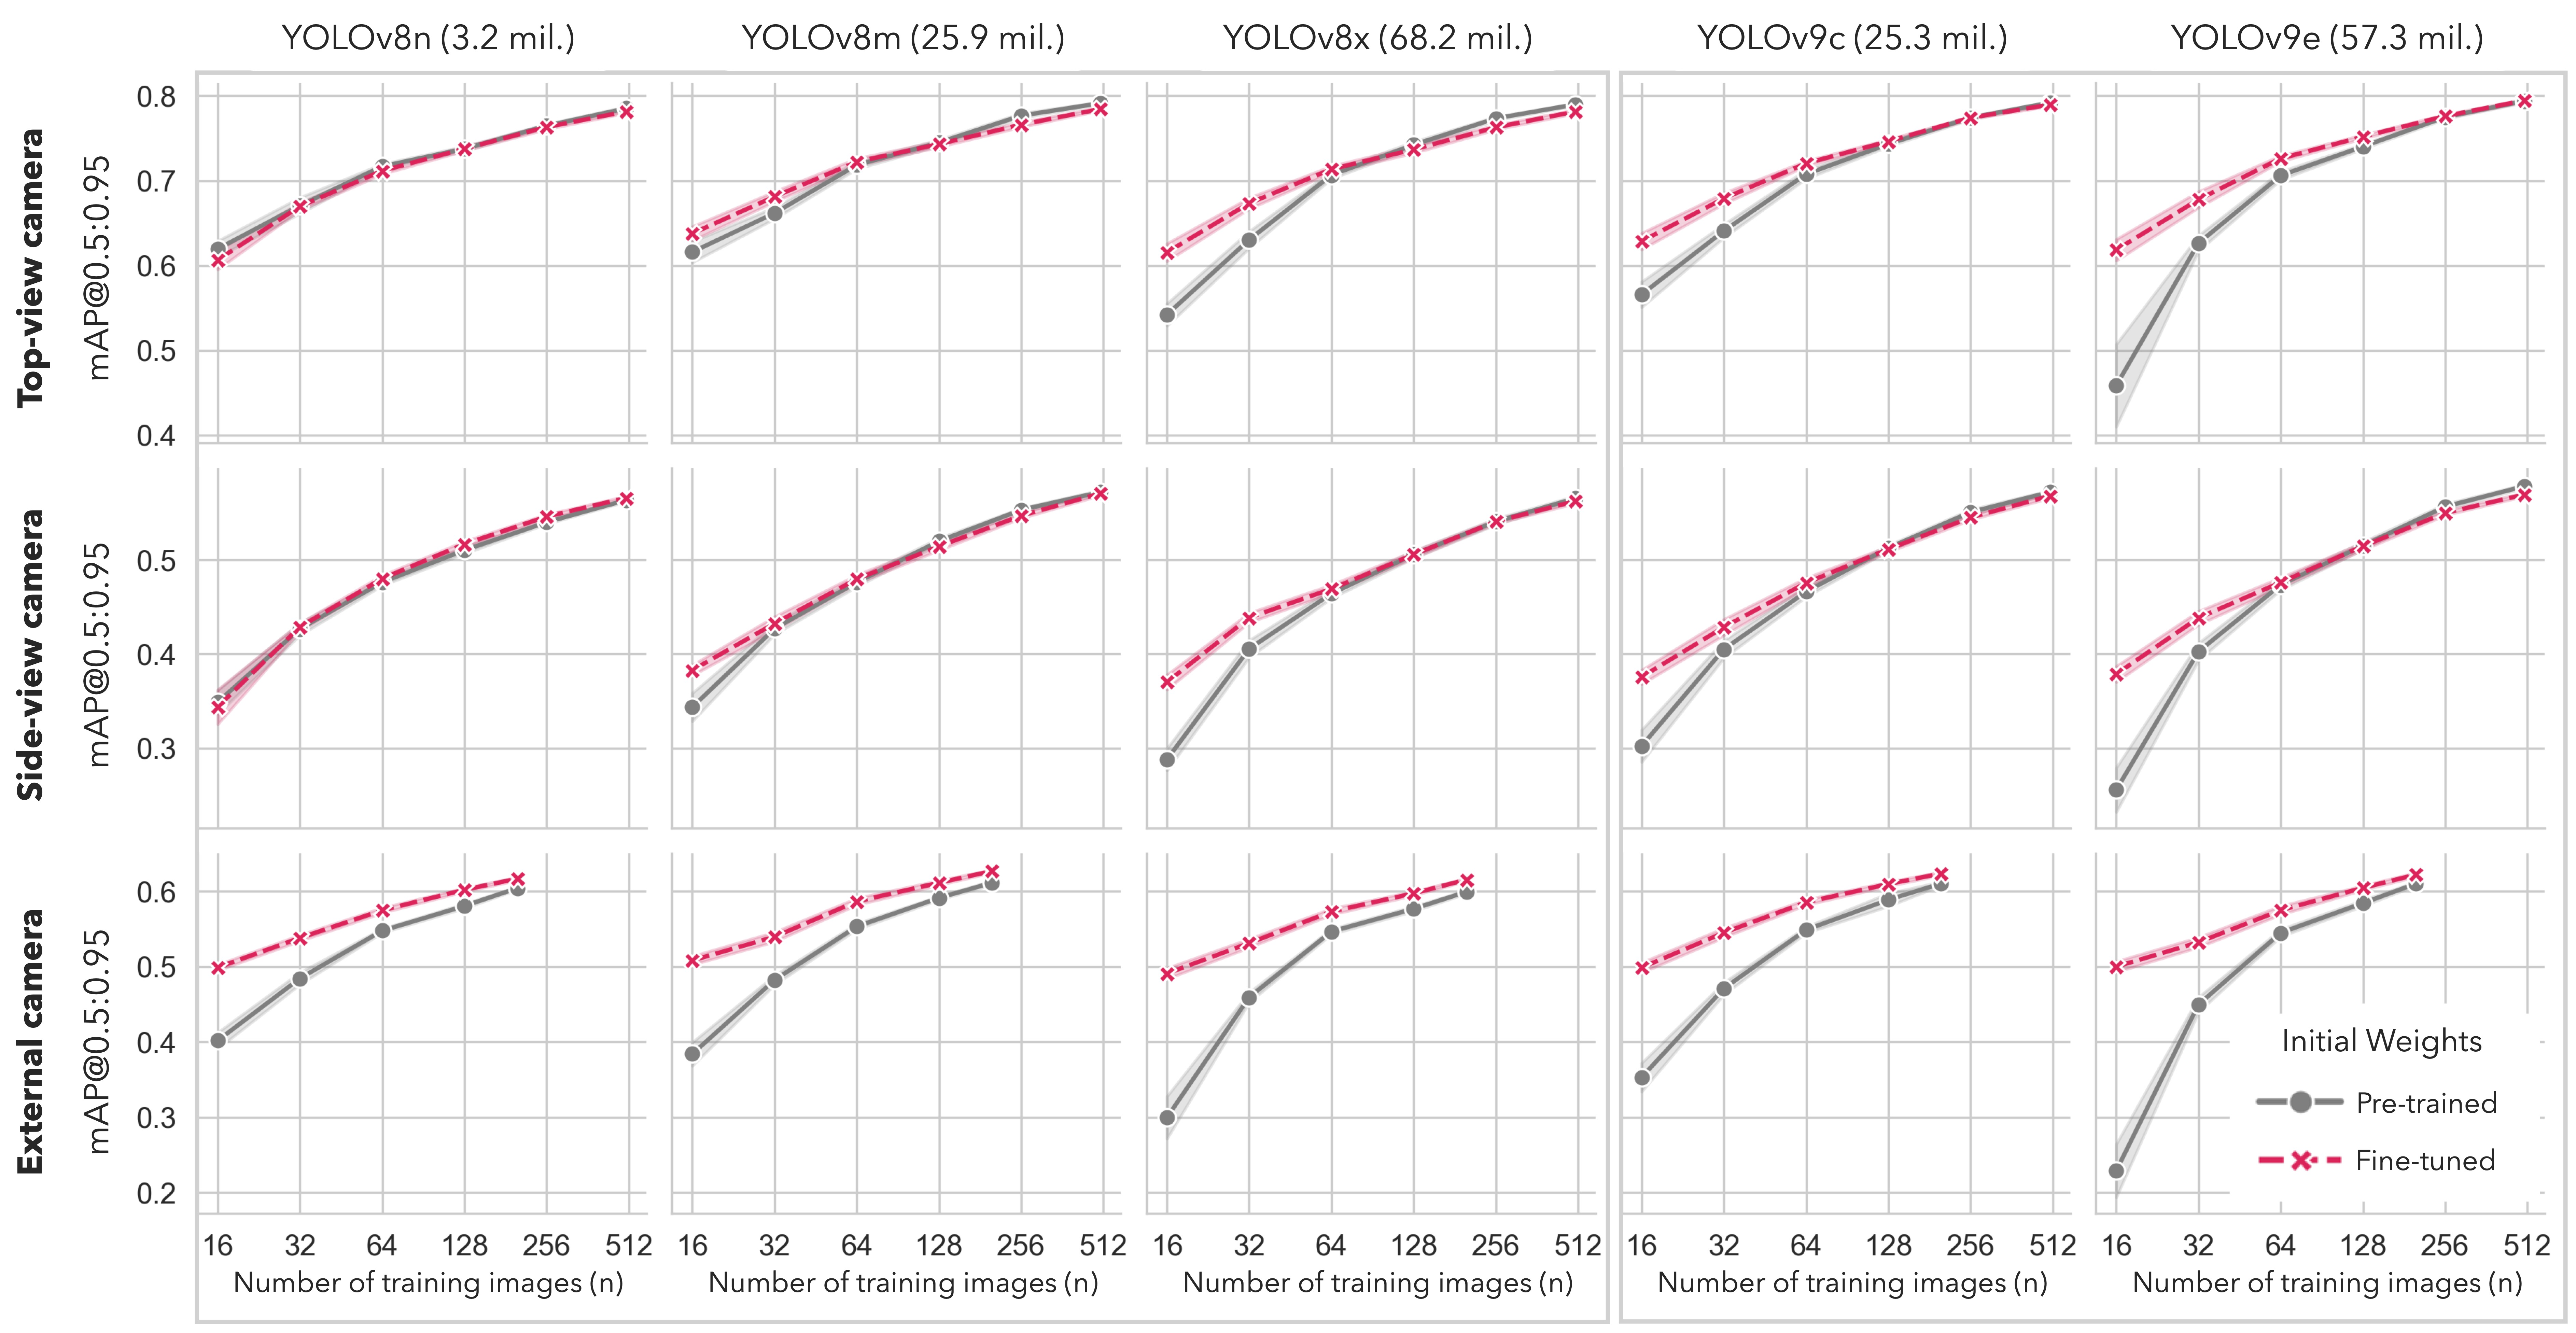
\includegraphics[width=1\textwidth]{figure_5.jpg}
    \caption{Varied generalization performance in $\text{mAP@{0.5:0.95}}$ with different initial weights. Red lines represent instances where weights were initialized with fine-tuned weights from other data configuration, while grey lines indicate scenarios employing pre-trained weights (i.e., trained with the COCO dataset). The horizontal axis indicates the number of training samples used for the fine-tuning procedure.}
    \label{fig:finetune}
\end{figure}

This study suggests that, for YOLO models with fewer parameters, such as YOLOv8n and YOLOv8m, the choice of weight initialization does not make a significant difference in fine-tuning performance. In contrast, larger models like YOLOv8x, YOLOv9c, and YOLOv9e exhibit improved performance when weights are initialized from a model that has been previously fine-tuned in a similar data configuration, as described in Table \ref{tab:fintune_config}. Therefore, when fine-tuning larger models with a limited dataset, it is beneficial to utilize weights previously fine-tuned on various data configurations. This approach leverages the additional learned features and adaptability from the initial fine-tuning, resulting in better performance even with a small amount of new data. For example, our results showed that YOLOv9e achieved optimal performance with fewer fine-tuning samples when initialized with fine-tuned weights compared to default weights. Conversely, for smaller models, the weight initialization strategy does not significantly impact fine-tuning performance. This is likely due to the lower complexity and fewer parameters of these models, which makes them less dependent on the initial weight configuration to achieve good performance. In practical terms, this means that for simpler models, researchers can save time and computational resources by directly fine-tuning without the need for customized weight initialization.

The analysis of Figure \ref{fig:finetune} also provides insight into performance across homogeneous viewpoint data configurations, specifically `Top-View Camera' and `Side-View Camera'. The data demonstrates that the `Top-View Camera' configuration consistently yields higher mAP values regardless of the training sample size and weight initialization conditions. This implies that the `Side-View Camera' configuration, where both training and test images are captured from the side view, presents a more formidable challenge for cow detection compared to the `Top-View Camera' configuration. The side view poses difficulties due to occlusions by neighboring cows and additional distractions, such as obstacles in aisles and fences. Furthermore, cows located further away in side-view images may not be as visible, complicating feature extraction. In contrast, the `Top-View Camera' configuration benefits from an unobstructed aerial perspective, ensuring that the top view of all cow instances is clearly visible and free from such obstructions. This distinction in visibility between the two configurations contributes to the ease of feature extraction and ultimately, the performance disparity observed.

These findings align with the results from Study 1, which demonstrated that changes in camera view angles dramatically affect model performance. In Study 1, we found that models trained on Top-View datasets struggled the most to detect cows from side-view images, with performance dropping by approximately 60\% in $\text{mAP@{0.5}}$. This significant drop in performance is attributed to the same reasons identified in Study 3: the side view introduces occlusions and distractions that are not present in the top view, making feature extraction more challenging. 

This study highlights that when working with external or unseen datasets, fine-tuning with custom initial weights trained on relevant tasks brings advantages to the detection tasks. On the other hand, simpler models do not benefit much from customized weights, suggesting that it is more efficient to train a simple model with pre-trained weights without relying on prior relevant information, which sometimes requires intensive labor efforts.


\subsection*{Computational Resource Requirements}

\begin{figure}[h]
    \centering
    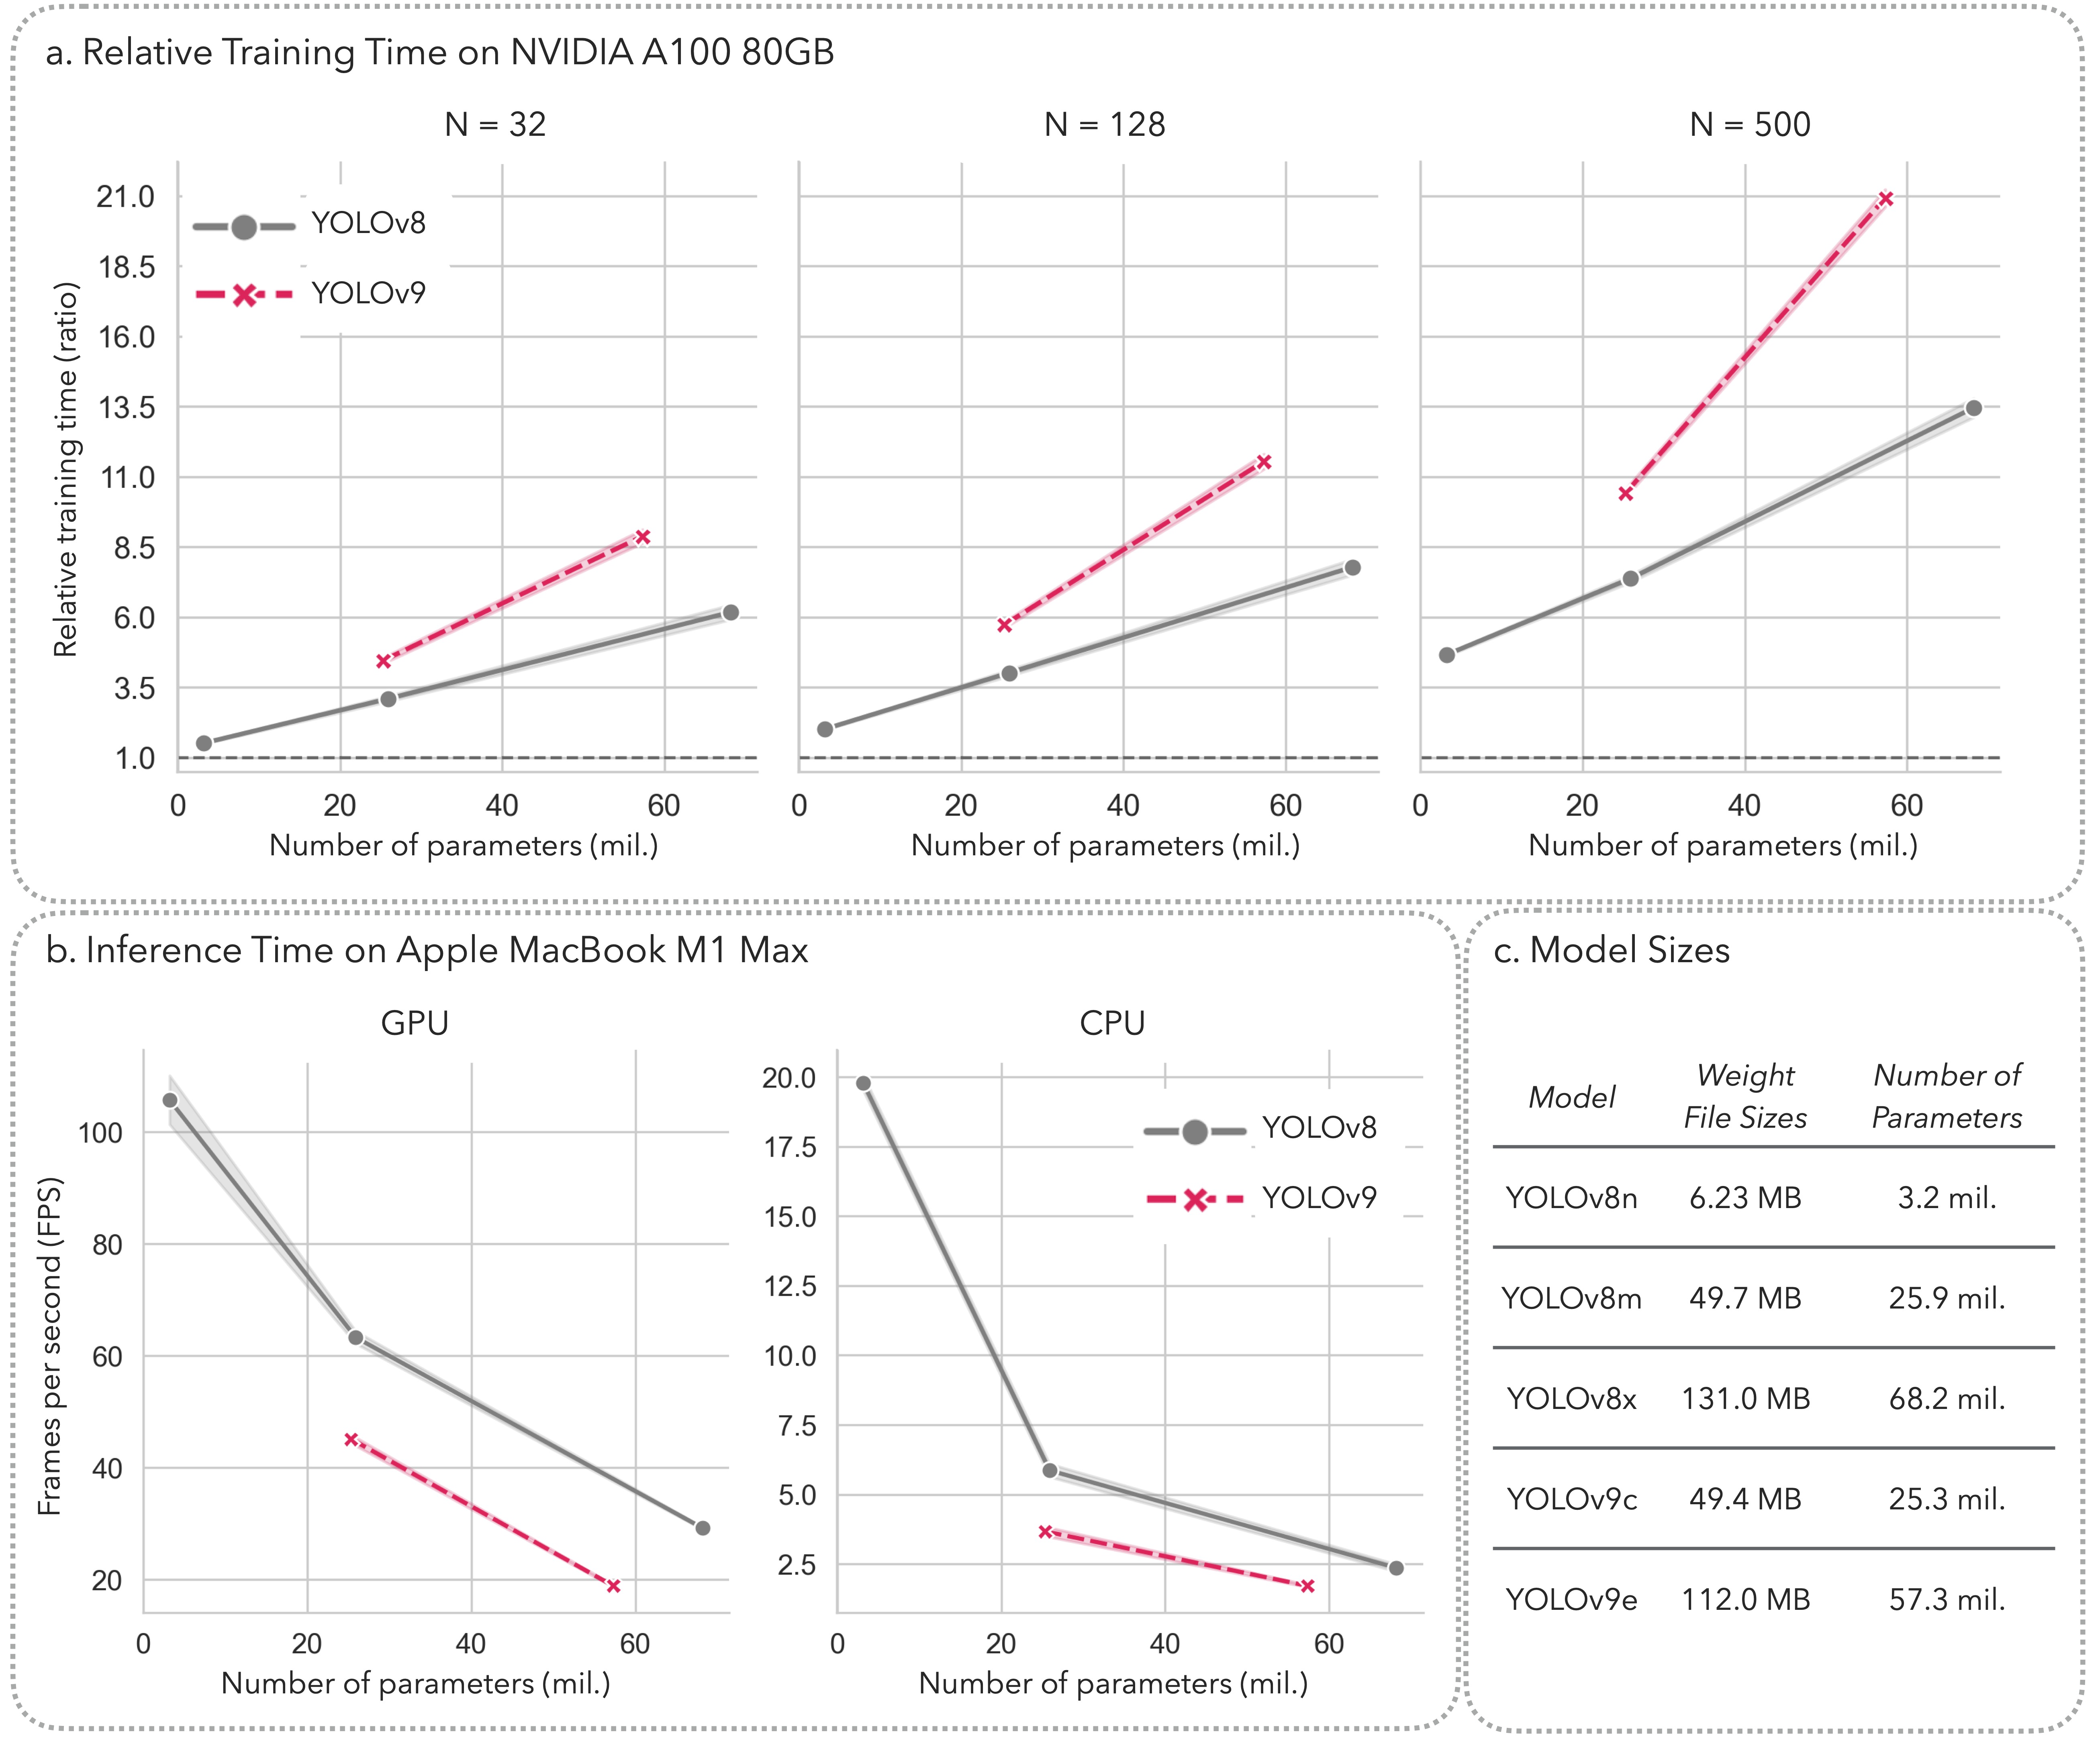
\includegraphics[width=.8\textwidth]{figure_6.jpg}
    \caption{Comparative evaluation of computational resource requirements. (a) Training time (expressed as a multiple of baseline time) versus number of parameters for YOLOv8 and YOLOv9 models, presented for training sample sizes of 32 (left), 128 (middle), and 500 (right). (b) Inference frequency versus number of parameters for YOLOv8 and YOLOv9 models on GPU (left) and CPU (right). (c) A table displaying the weight sizes and parameter counts of various YOLOv8 and YOLOv9 models.}
    \label{fig:resources}
\end{figure}

The evaluation of computational resource requirements is crucial for understanding the feasibility of deploying YOLO models in real-world applications, especially in environments with limited computational resources. This section compares training time (Figure \ref{fig:resources}a), inference time (Figure \ref{fig:resources}b), and model weight sizes (Figure \ref{fig:resources}c) for various YOLO models.

The training time for each model was measured and expressed as a multiple of the baseline training time, which is the time required to train the YOLOv8n model with 32 samples. The results indicated that using the largest model, YOLOv8x, which has 20 times more parameters, increased training time by 4 to 6 times, depending on the training sample size. Additionally, the YOLOv9 models generally required more training time and had slower inference frames per second (FPS) compared to the YOLOv8 models. The gap in training time expanded as the number of training samples increased.

Inference time was measured as the average FPS in a batch of 64 images. Running the models on a CPU with the smallest model (YOLOv8n) was slower than running the largest model (YOLOv8x) on a GPU. For example, the FPS for the small, YOLOv8n, on a CPU was 19.77, while the FPS for YOLOv8x on a GPU was 29.21. High FPS models are essential for real-time inference, which usually requires a model with an FPS higher than 30. The results indicate that implementing YOLO models on a CPU may not meet real-time requirements, especially for larger models.

Lastly, model weight sizes were also considered, impacting memory requirements and deployment feasibility, especially in edge computing environments. The weight sizes and parameter counts of various YOLO models are displayed in Figure \ref{fig:resources}c.

In conclusion, this evaluation highlights the trade-offs between model complexity and computational efficiency. The larger YOLO models, while offering potentially better performance, require significantly more computational resources. This analysis helps researchers and practitioners select the appropriate model based on the available computational resources and the specific requirements of their application.

\section{Conclusion}

This study examined the impact of various training configurations and model complexities on the performance of YOLOv8 and YOLOv9 models for cow detection in indoor farm environments. Our results indicate that model performance is highly dependent on camera viewpoints, with side views presenting the greatest challenges. Additionally, fine-tuning models with weights from similar datasets substantially enhances performance, particularly for complex models in scenarios with limited data. We also introduce a public cow localization dataset, 'COLO', to support the research community.

The findings indicate that while increasing model complexity can improve performance, this is not always the case, especially in challenging configurations like 'Top2Side', which predict images from a side view using a model trained on top-view images. Models trained on a single viewpoint exhibit limited generalization, underscoring the importance of incorporating diverse and consistent camera angles in the training data.

Despite the promising results, this study has certain limitations. The models' performance was evaluated under specific indoor farm conditions, which may not generalize to all livestock environments. Moreover, the reliance on pre-defined configurations may limit the applicability of our findings to more dynamic settings.

Future work should explore adaptive methods for enhancing model generalization across varied viewpoints and environmental conditions. Additionally, investigating the integration of advanced data augmentation techniques and more diverse datasets could further improve detection accuracy and robustness.

In conclusion, this study offers practical insights into reproducing model performance in new environmental settings and provides the public 'COLO' dataset to facilitate further research and advancements in the field.